\documentclass[12pt,a4paper]{article}
\usepackage[a4paper,top=1.5cm, bottom=1.5cm, left=1.5cm, right=1.5cm]{geometry}
\usepackage[T2A]{fontenc}
\usepackage[utf8]{inputenc}
\usepackage[russian]{babel}
\usepackage{amsmath}
\usepackage{amssymb}
\usepackage{graphicx}
\usepackage{floatrow}
\usepackage{booktabs}
\usepackage{wrapfig}
\usepackage{indentfirst}
\usepackage{lipsum}
\usepackage{subcaption}
\usepackage{float}
\usepackage{enumitem}
\restylefloat{table}

\newcommand{\figref}[1]{(см. рис. \ref{#1})}
\newcommand{\e}[1]{\text{$\cdot10^{#1}$}}

\title{Лабораторная работа 3.3.4\\ Эффект Холла в полупроводниках}
\author{Симанкович Александр \\ Б01-104}
\date{07.09.2022}

\begin{document}
	\maketitle
	
	\section*{Аннотация}
	
	В работе нашла экспериментальное подтверждение гипотеза о возникновении поперечной ЭДС в проводнике с током, помещенном в магнитное поле (эффект Холла). Измерен коэффициент пропорциональности между ЭДС Холла и магнитной индукцией, определены подвижность и концентрация основных носителей заряда в кристаллическом Ge.
		
	\section*{Теоретическое введение}
	
	В электрическом поле $\vec{E}$ на заряды действует сила $q\vec{E}$. Во внешнем магнитном поле $\vec{B}$ на движущиеся заряды также действует сила Лоренца. Результирующая сила:
	
	$$ \vec{F} = q\vec{E} + q\vec{u} \times \vec{B}.$$
	
	Эта сила вызывает движение носителей, направление которого в общем случае не совпадает с $\vec{E}$. Действительно, траектории частиц будут ли­бо искривляться, либо, если геометрия проводника этого не позволя­ет, возникнет дополнительное электрическое поле, компенсирующее маг­нитную составляющую силы Лоренца. Возникновение поперечного току электрического поля в образце, помещённом во внешнее магнитное поле, называют эффектом Холла.
	
	\begin{figure}[h]
		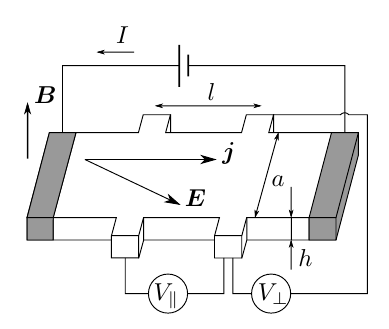
\includegraphics[scale=0.65]{res/scheme_hall.png}
		\caption{Схема мостика Холла}
		\label{scheme_hall}
	\end{figure}

	В работе для проверки эффекта Холла используется мостик Холла \figref{scheme_hall}.
	
	В мостике Холла реализовывается простой случай, когда направление тока ($\vec{j} \parallel \vec{x}$) перпендикулярно направлению внешнего магнитного поля ($\vec{B} \parallel \vec{z}$). На один носитель тока со стороны магнитного поля действует сила $F_y = - q u_x B_z$. После установления стационарного режима носители перераспределены так, что создают поле $E_y = - \frac{F_y}{q} = u_x B_z = \frac{j_x}{nq} B_z$. Напряжение, появившееся вследствие перераспределения зарядов, называется холловским:
	$$ U_\perp = E_y a = \frac{j_x B_z}{n q} a. $$
	
	Учитывая, что $j_x = \frac{I}{ah}$, получаем:
	
	\begin{equation}
		\label{U_perp}
		U_\perp = \frac{B_z}{nqh} \cdot I = R_H \cdot \frac{B_z}{h} \cdot I,
	\end{equation}
	где $R_H = \frac{1}{nq}$ -- постоянная Холла.
	
	Для продольной составляющей напряжения выполняется закон Ома. Из него получаем:
	
	$$ U_\parallel = E_x l = \frac{j_x}{\sigma_0} l = I R_0, $$
	где $R_0 = \frac{l}{\sigma_0 a h}$.
	
	\begin{equation}
		\label{sigma_0}
		\sigma_0 = \frac{I \cdot l}{U_{35} \cdot h \cdot a}.
	\end{equation}
	
	
	\section*{Методика эксперимента}
	
	\subsection*{Оборудование и приборы}
	\begin{itemize}[itemsep = 0pt, parsep=0pt]
		\item электромагнит с регулируемым источником пи­тания GPR-11H30D ($A_1$);
		\item вольтметр B7-78/1;
		\item миллиамперметр M2020 ($A_2$);
		\item милливеберметр M119 и мил­литесламетр AKTAKOM ATE-8702;
		\item источник питания (1,5 В);
		\item образцы легированного германия;
	\end{itemize}
	
	\begin{figure}[h]
		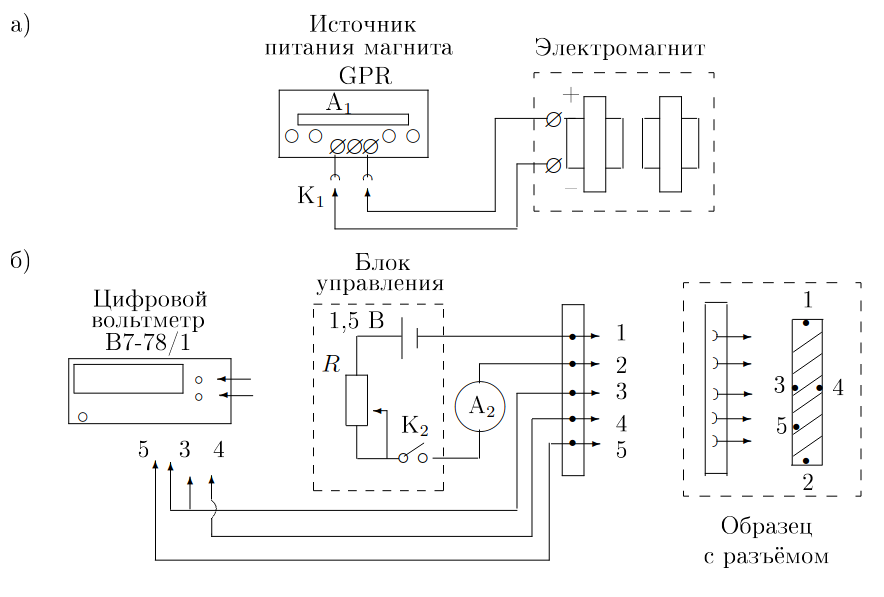
\includegraphics[scale=0.65]{res/scheme.png}
		\caption{Схема установки для исследования эффекта Холла в полупроводниках}
		\label{scheme}
	\end{figure}
	
	В зазоре электромагнита \figref{scheme} создаётся постоянное магнитное поле, величину которого можно менять с помощью регуля­тора источника питания электромагнита. Ток питания электромагни­та измеряется амперметром $A_1$.
	
	Градуировка электромагнита проводится при помощи милливеберметра и миллитесламетра.
	
	Прямоугольный образец из легированного германия, смонтирован­ный в специальном держателе \figref{scheme}, подключается к источнику пита­ния ($\approx$ 1,5 В). При замыкании ключа $K_2$ вдоль длинной стороны образца (контакты 3, 5) течёт ток, величина которого регулируется реостатом $R_2$ и измеряется миллиамперметром $A_2$.
	
	В образце с током, помещенном в зазор электромагнита, между контактами 3 и 4 возникает разность потенциалов $U_{34}$, которая измеряется с помощью цифрового вольтметра.
	
	Контакты 3 и 4 вследствие неточности подпайки могут не лежать на эквипотенциали, для устранения этого эффекта будем измерять начальное значение напряжения $U_0$ (при выключенном магните) в каждой серии измерений.

	\section*{Результаты}
	
	\subsection*{Градуировка электромагнита}
	
	Проведем градуировку электромагнита. Для этого измерим зависимость $B(I)$, где $B$ -- модуль вектора индукции магнитного поле в зазоре, $I_M$ -- ток, протекающий через обмотки магнита. Измерения проведем милливеберметром M119 и миллитесламетром AKTAKOM ATE-8702. Погрешности данных приборов:
	
	$$ \varsigma_{\text{Вб}} = 0.15 \; \text{мВб} \quad \varepsilon_{\text{Тл}} = 0.06 $$
	
	Точность измерения $I_M$ определяется точностью амперметра $A_1$, встроенного в лабораторный блок питания GPR-11H30D: $$\varsigma_{A_1} = 0.005 \; \text{А}$$
	
	%\begin{table}[H]
	%	\input{gen/electromagnet.tex}
	%	\caption{Результаты измерений индукции магнита}
	%\end{table}

	Построим графики $B(I)$ по результатам измерения магнитного поля милливеберметром и миллитесламетром.
	
	\begin{figure}[H]
		\includegraphics[scale=1]{gen/electromagnet_BI.pdf}
		\caption{$B(I_M)$}
	\end{figure}

	Как видно из графика, данные веберметра и тесламетра расходятся. Тесламетр является более современным и тщательно откалиброванным прибором, тогда как данные веберметра могут зависеть от сопротивления соединительных проводов и наводок в них. По этой причине для последующих измерений выбираем калибровку тесламетром.
	
	\subsection*{ЭДС Холла}

	Проведем измерения $U_{34}(I_M)$ для различных $I$. Рассчитаем значения $B$ и занесем в таблицу.
	Измерения $I$ делаются миллиамперметром $A_2$, модель M2020: $\varsigma_{A_2} = 5 \; \text{мкА} $.
	Измерения $U$ проводятся вольтметром $V_1$, модель B7-78/1: $\varsigma_{V_1} = 3.5 \; \text{мкВ}$.
	В измерениях учитывается $U_0$ -- сдвиг напряжения при нулевом магнитном поле, возникающий из-за неточности подпайки.
	
	%\begin{table}[H]
	%	\addtolength{\tabcolsep}{-4pt}
	%	\footnotesize
	%	\input{gen/hallEMF_UI.tex}
	%	\caption{Результаты измерений $U_{34}(I_M)$}
	%\end{table}
	
	%\begin{table}[H]
	%	\addtolength{\tabcolsep}{-4pt}
	%	\footnotesize
	%	\input{gen/hallEMF_UB.tex}
	%	\caption{$U_{34}(B)$}
	%\end{table}
		
	\begin{figure}[H]
		\includegraphics{gen/hallEMF_UB.pdf}
		\caption{Зависимость холловского напряжения от индукции магнитного поля}
	\end{figure}

	По методу наименьших квадратов рассчитаем параметры графиков, считая зависимость линейной. В результате получим значение углового коэффициента $K = \frac{\Delta \mathcal{E}_H}{\Delta B}$ для каждого графика. Построим график $K(I)$ и рассчитаем его параметры.
	
	\begin{figure}[H]
		\includegraphics{gen/hallEMF_KI.pdf}
		\caption{Зависимость углового коэффициента от тока через образец}
	\end{figure}
	
	\begin{table}[h]
		\caption{$K(I)$}
		\input{gen/hallEMF_KI.tex}
	\end{table}
	
	\begin{table}[h]
		\caption{Параметры графика $K(I)$}
		\input{gen/hallEMF_KI_mnk.tex}
	\end{table}

	Выясним знак носителей заряда в легированном германии. Мы знаем, что электрическое поле направлено от $4$ к $3,5$ из знака напряжения на вольтметре $V1$. Воспользовавшись правилом буравчика и правилом левой руки получим, что сила Лоренца направлена от $4$ к $3,5$ для обоих знаков зарядов. Следовательно, носители заряда в легированном германии имеют положительный заряд (дырочная проводимость).
	
	\begin{figure}[H]
		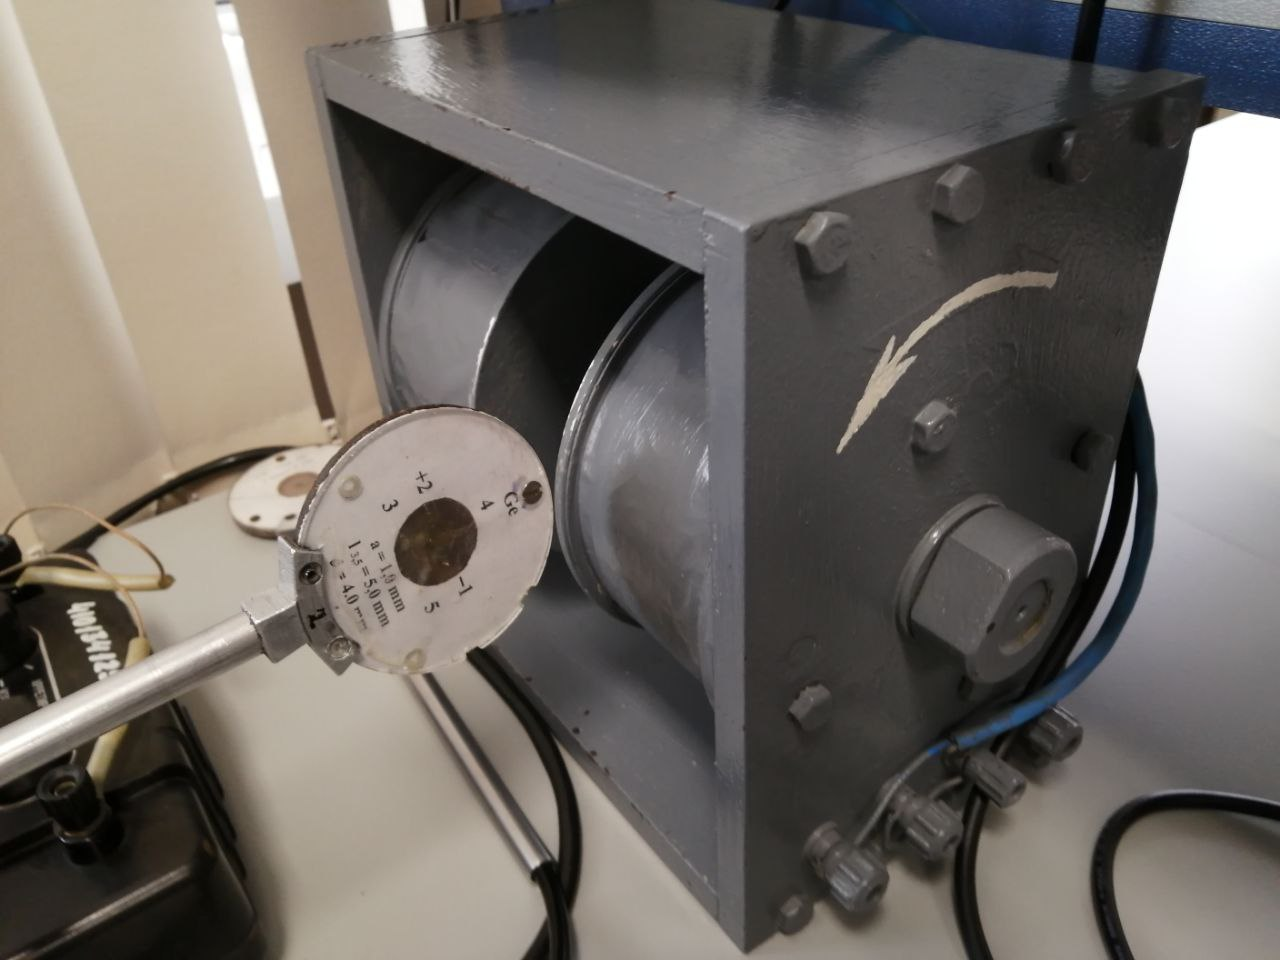
\includegraphics[scale = 0.25]{res/probe_coil.jpg}
		\caption{Пробная катушка и ее положение относительно магнита}
	\end{figure}
	
	Определим коэффициент Холла $R_H$ по формуле \eqref{U_perp}:
	$$ R_H = h \frac{U_\perp}{BI} = h \cdot a_K = 1.0 \; \text{мм} \cdot 0.672 \; \frac{\text{В}}{\text{Тл} \cdot \text{А}} = (6.7 \pm 0.4) \cdot 10^{-4} \; \frac{\text{м}^3}{\text{Кл}} $$
	
	Определим концентрацию $n$:
	$$ n = \frac{1}{R_H e} = (9.3 \pm 0.4) \cdot 10^{21} \frac{1}{\text{м}^3} $$
	
	\subsubsection*{Альтернативный метод обработки}
	
	Также для определения искомого параметра можно воспользоваться тем, что:
	$$ \mathcal{E}_H = \frac{R_H}{h} \cdot BI $$
	
	Построим график $\mathcal{E}_H (BI)$ и определим его параметры.
	
	\begin{figure}[H]
		\includegraphics[]{gen/hallEMF_UIB.pdf}
		\caption{Зависимость холловского напряжения от произведения индукции поля и тока в образце}
	\end{figure}
	
	\begin{table}[h]
		\caption{Параметры графика $\mathcal{E}_H (IB)$}
		\input{gen/hallEMF_UIB_mnk.tex}
	\end{table}

	Определим коэффициент Холла $R_H$ по формуле \eqref{U_perp}:
	$$ R_H = h \frac{U_\perp}{BI} = h \cdot a_{IB} = 1.0 \; \text{мм} \cdot 0.689 \; \frac{\text{В}}{\text{Тл} \cdot \text{А}} = (6.9 \pm 0.4) \cdot 10^{-4} \; \frac{\text{м}^3}{\text{Кл}} $$
	
	Определим концентрацию $n$:
	$$ n = \frac{1}{R_H e} = (9.1 \pm 0.5) \cdot 10^{21} \frac{1}{\text{м}^3} $$
	
	\subsection*{Удельная проводимость}
	
	Измерим $U_{35} (I)$ в образце. Построим график $U_{35} (I)$ и рассчитаем его параметры.
	
	%\begin{table}[h]
	%	\caption{Результаты измерений $I(U_{35})$}
	%	\input{gen/cond_UI.tex}
	%\end{table}
	
	\begin{figure}[H]
		\includegraphics{gen/cond_UI.pdf}
		\caption{Зависимость напряжения $U_{35}$ от основного тока в образце}
	\end{figure}
	
	\begin{table}[h]
		\caption{Параметры графика $U_{35} (I)$}
		\input{gen/cond_UI_mnk.tex}
	\end{table}
	
	Рассчитаем удельную проводимость $\sigma_0$:
	$$ \sigma_0 = \frac{I \cdot l}{U_{35} \cdot h \cdot a} = \frac{ 5.0 \; \text{мм} }{ 4.04 \; \text{Ом} \cdot 1.0 \; \text{мм} \cdot 4.0 \; \text{мм}} = (309 \pm 27) \frac{1}{\text{Ом} \cdot \text{м}} $$
	
	Рассчитаем подвижность зарядов $b$:
	$$ b = \frac{\sigma_0}{e n} = (2230 \pm 220) \frac{\text{см}^2}{\text{В} \cdot \text{с}} $$
	
	\section*{Заключение и выводы}
	
	Данная работа подтверждает существование эффекта Холла в полупроводниках.
	
	Получено значение коэффициента Холла $ R_H = (6.9 \pm 0.4) \cdot 10^{-4} \; \frac{\text{м}^3}{\text{Кл}} $. Также в работе оценено значение концентрации носителей тока в образце $ n = (8.7 \pm 0.4) \cdot 10^{21} \; \frac{1}{\text{м}^3} $, удельная проводимость $ \sigma_0 = (309 \pm 27) \; \frac{1}{\text{Ом} \cdot \text{м}} $, подвижность носителей $ b = \frac{\sigma_0}{e n} = (2230 \pm 220) \; \frac{\text{см}^2}{\text{В} \cdot \text{с}} $.
	
	Справочные данные для данного образца германия отсутствуют, большинство параметров зависят от степени легирования. Значения подвижности носителей зависит от легирующего элемента и лежат в пределах\footnote{Эффект Холла в германии, легированном разными примесями, Г. П. Гайдар, Е. Ю. Гайворонская, 2017} $(2000 \div 3000) \; \frac{\text{см}^2}{\text{В} \cdot \text{с}}$.
	
\end{document}